\documentclass[a4paper, 10pt]{article}
\usepackage[margin=0.5in]{geometry}
\usepackage{comment} % enables the use of multi-line comments (\ifx \fi) 
\usepackage{lipsum} %This package just generates Lorem Ipsum filler text. 
\usepackage{fullpage} % changes the margin
\usepackage{multirow}	
\usepackage{amssymb}
\usepackage{amsmath}
\usepackage{graphicx}
\usepackage{listings}
\usepackage{hyperref}
\newcommand\tab[1][1cm]{\hspace*{#1}}
\newcommand{\norm}[1]{\left\lVert#1\right\rVert}
\newcommand{\p}[1]{\left(#1\right)}
\newcommand{\bk}[1]{\left[#1\right]}
\newcommand{\bc}[1]{ \left\{#1\right\} }
\newcommand{\abs}[1]{ \left|#1\right| }
\newcommand{\mat}{ \begin{pmatrix} }
\newcommand{\tam}{ \end{pmatrix} }
\newcommand{\suml}{ \sum_{i=1}^n }
\newcommand{\prodl}{ \prod_{i=1}^n }
\newcommand{\ds}{ \displaystyle }
\newcommand{\df}[2]{ \frac{d#1}{d#2} }
\newcommand{\ddf}[2]{ \frac{d^2#1}{d{#2}^2} }
\newcommand{\pd}[2]{ \frac{\partial#1}{\partial#2} }
\newcommand{\pdd}[2]{ \frac{\partial^2#1}{\partial{#2}^2} }
\newcommand{\N}{ \mathcal{N} }
\newcommand{\E}{ \text{E} }
\begin{document}
%Header-Make sure you update this information!!!!
\noindent
\textbf{STAT 222 Homework \#2} \hfill \textbf{Mary Silva}\\
UCSC \hfill  30 April 2020\\
\\
\begin{enumerate}
    
    \item[\textbf{1.}] \textbf{Posterior Inference for one sample problems using DP priors}
    
        Consider data = $(y_1, ..., y_n)$, and the following DP-based nonparametric model:
        
        \begin{align*}
            Y_i|G &\stackrel{iid}{\sim} \ G, \quad i = 1, ... ,n \\
            G &\sim DP(\alpha,G_0) \\
        \end{align*}
        with $G_0 = N(m, s^2)$ for fixed $m, s^2,$ and  $\alpha$. 
        
        The objective here is to use simulated data to study posterior inference results for $G$ under different prior choices for $M$ and $G_0$, different underlying distributions that generate the data, and different sample sizes. In particular,  consider:
        
        \begin{itemize}
            \item two data generating distributions: 1) a N(0; 1) distribution, and 2) the mixture of normal distributions which yields a bimodal c.d.f. with heavy right tail,
           $$0.5 N(-2.5, \ 0.5^2) + 0.3 N(0.5, \ 0.7^2) + 0.2 N(1.5,\ 2^2)$$
           \item sample sizes n = 20, n = 200, and n = 2000.
        \end{itemize}
        % Discuss prior specification for the DP prior parameters $m, s^2$. For each of the 6 data sets corresponding to the combinations above, obtain posterior point and interval estimates for the c.d.f. $G$ and discuss how well the model fits the data. Perform a prior sensitivity analysis to study the effect of $m, s^2, \alpha$ on the posterior estimates for $G$.
    
    \item[\textbf{SOLUTION}: ]
    In order to simulate from the posterior distribution, Ferguson's definition of the DP is used. In the first case we draw samples from a $N(0,1)$ distribution, with a sample size of 20, 200, and 2000. For each simulation I will generate 10 posterior samples. The hyperparameters $m$ and $s^2$ are chosen to be the sample mean and sample standard deviation of each data sample.
    
    \begin{figure}[h!]
        \centering
        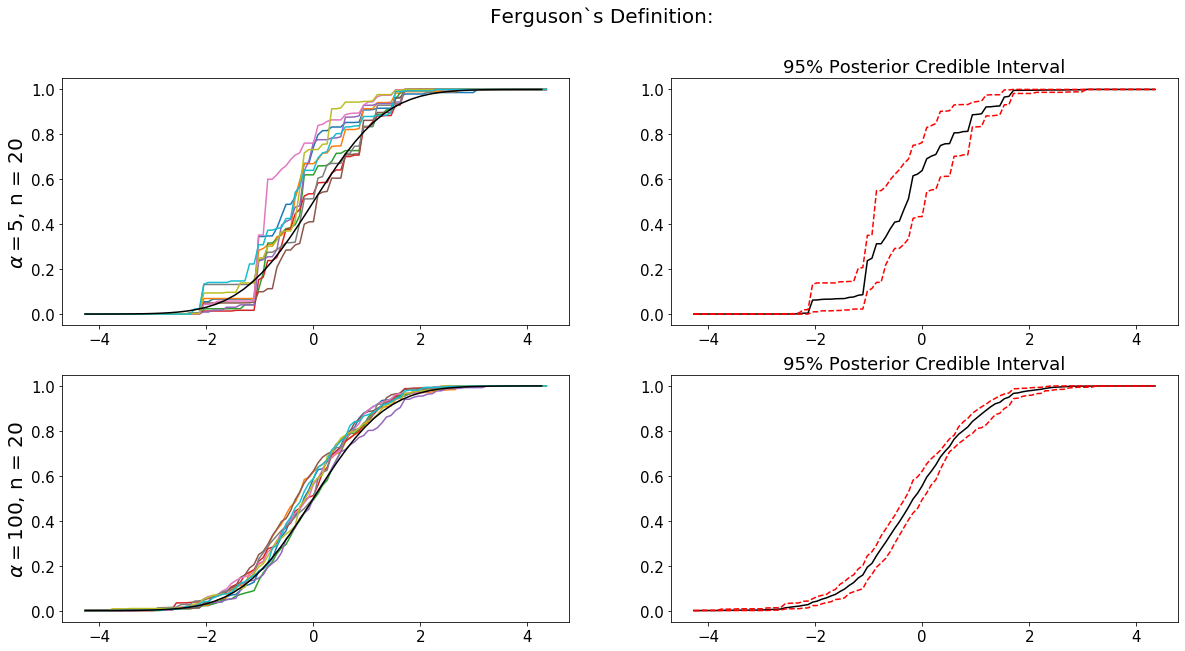
\includegraphics[scale = 0.4]{hw1a_20.png}
        \caption{Ferguson's definition of the DP drawb from a N(0,1) distribution with a sample size of 20 and $\alpha = 5$ (top) and $\alpha = 100$ (bottom). The right is the corresponding $95\%$ posterior credible interval.}
        \label{1a20}
    \end{figure}
    \footnote{Code available at \url{https://github.com/msilva00/BNP_Homework/blob/master/HW2/HW2_Prob1.ipynb}.}
    \clearpage
    From Figure \ref{1a20}, changing $\alpha$ changes the posterior distributions, because the dataset is too small to condition the posteriors to become more similar to the normal distribution. It’s like if we are forcing the normal behaviour of the posterior by increasing our confidence in the normal prior and decrease our confidence in the data. We also see, larger $\alpha$ leads to a smaller $95\%$ posterior credible interval. This is due to the decrease of the variance as $\alpha$ gets larger.
    
    \begin{figure}[h!]
        \centering
        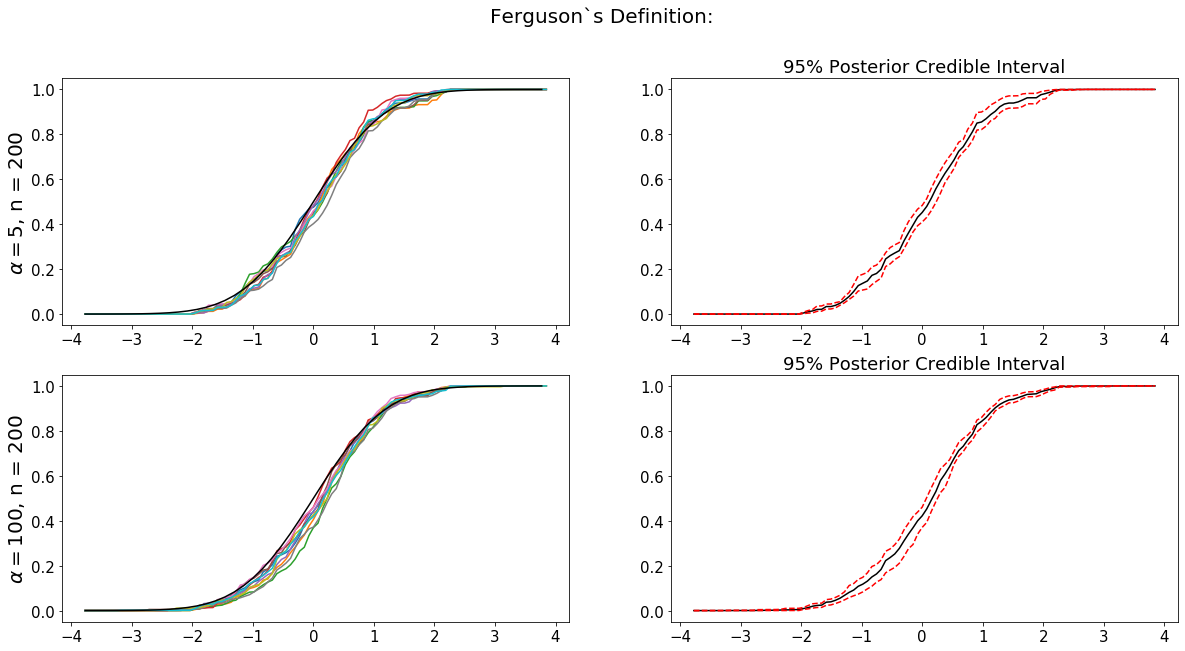
\includegraphics[scale = 0.35]{hw1a_200.png}
        \caption{Ferguson's definition of the DP drawb from a N(0,1) distribution with a sample size of 200 and $\alpha = 5$ (top) and $\alpha = 100$ (bottom). The right is the corresponding $95\%$ posterior credible interval.}
        \label{1a200}
    \end{figure}
    
    \begin{figure}[h!]
        \centering
        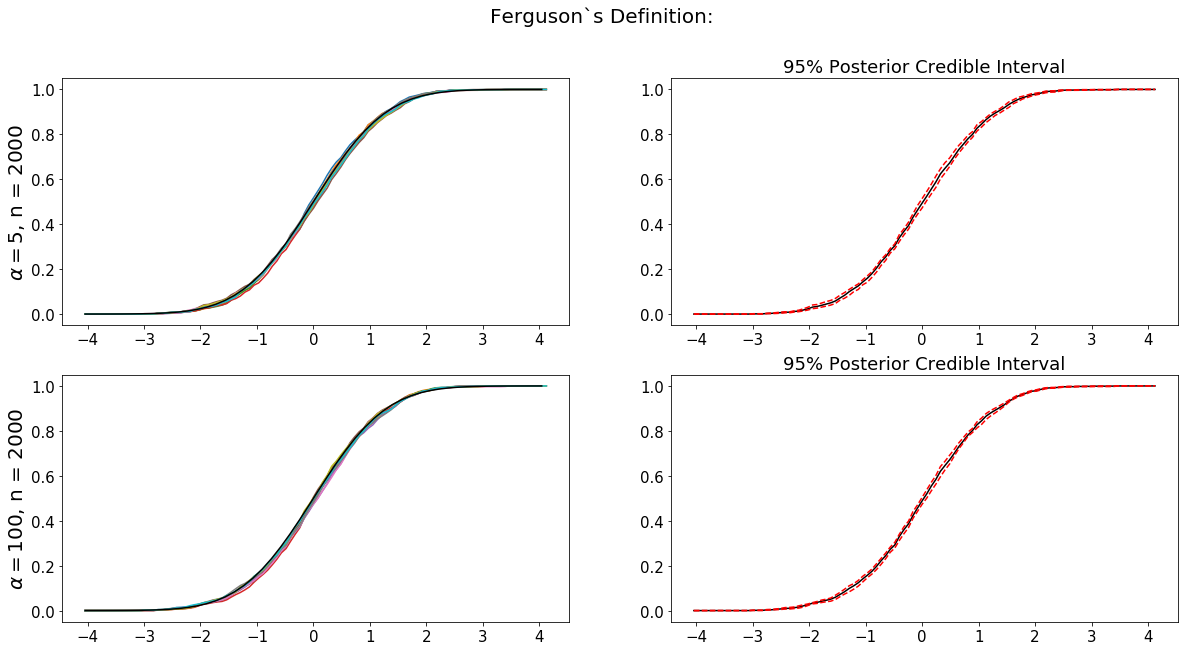
\includegraphics[scale = 0.35]{hw1a_2000.png}
        \caption{Ferguson's definition of the DP drawb from a N(0,1) distribution with a sample size of 2000 and $\alpha = 5$ (top) and $\alpha = 100$ (bottom). The right is the corresponding $95\%$ posterior credible interval.}
        \label{1a2000}
    \end{figure}
    
    Based on Figures \ref{1a200}-\ref{1a2000}, the effect of $\alpha$ is negligible because the simulated data is already producing a normal behavior to the posterior distribution. Also, the credible intervals don't change too much as $\alpha$ grows.
    \clearpage
    Now, we will use data that comes from a finite mixture of normal distributions. We simulate the ``true" distribution and plot the density using 20000 samples from the mixture and use it to compare the results.
    \begin{figure}[h!]
        \centering
        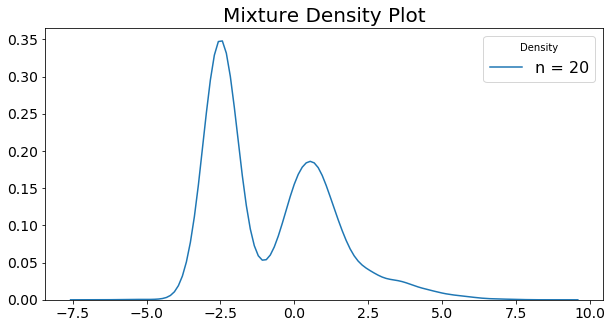
\includegraphics[scale = 0.37]{hw1b_truedens.png}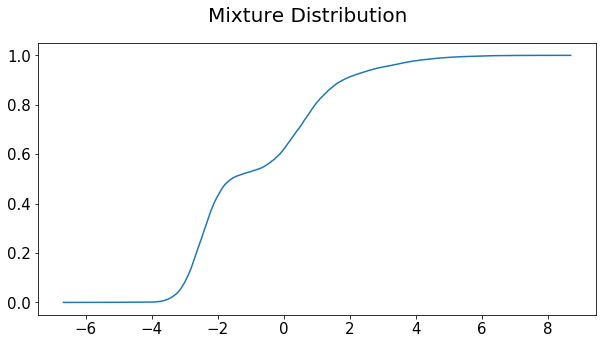
\includegraphics[scale=0.37]{hw1b_truedistr.png}
        \caption{Density for 20000 samples from the mixture of normal.}
        \label{nmix_dist}
    \end{figure}
    
    Next, we simulate from the posterior distribution using Ferguson's definition of the DP for simulated data with sample sizes $n=20, 200$, and $2000$, respectively.
    
    \begin{figure}[h!]
        \centering
        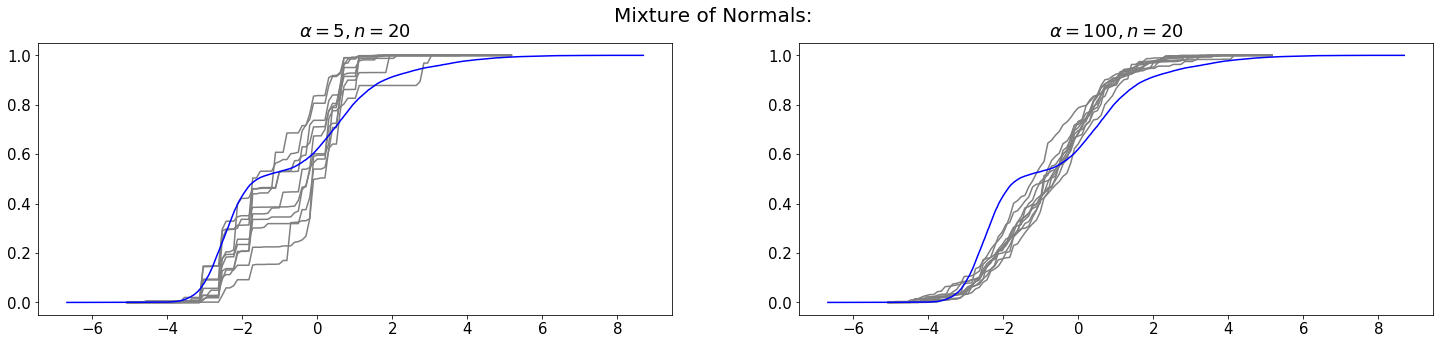
\includegraphics[scale = 0.33]{hw1b_20.png}
        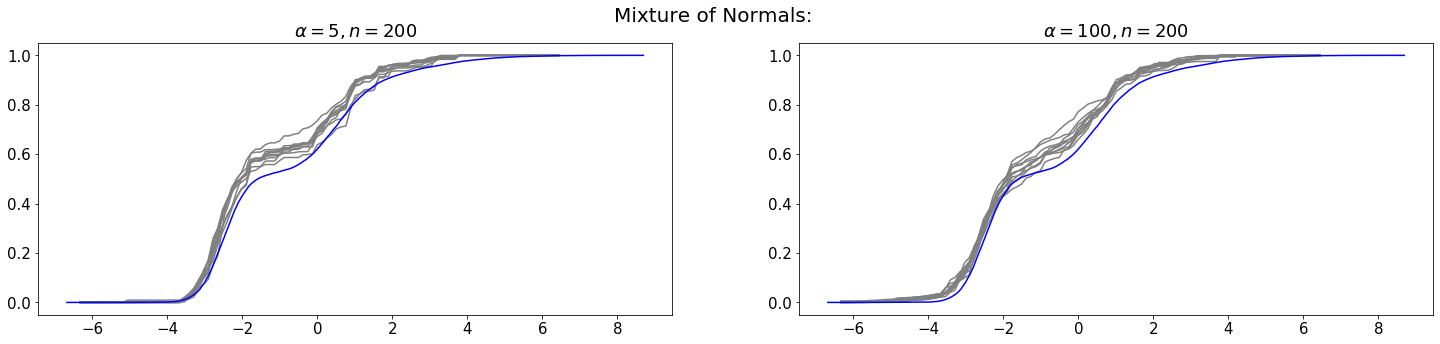
\includegraphics[scale = 0.33]{hw1b_200.png}
        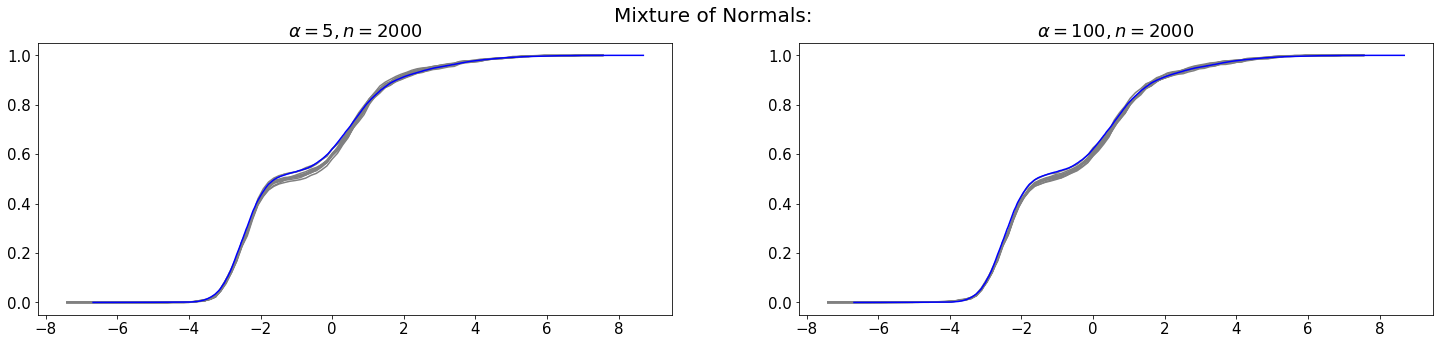
\includegraphics[scale = 0.33]{hw1b_2000.png}
        \caption{For each plot, we use sample datasets with $n=20$(top), $n=200$(middle), and $n = 2000$ (bottom) and use $\alpha = 5$(left) and $\alpha = 100$(right). The hyperparameters of the prior normal distribution are chosen based on the mean and sample standard deviation of each dataset. The grey lines represent posterior realizations from the DP, and the blue line represents the ``true" mixture density (the 20000 samples from the mixture distribution).}
        \label{1b_posterior}
    \end{figure}
    
    \clearpage
    \item[\textbf{2.}] \textbf{Posterior inference for count data using MDP priors}
    We consider again modeling a single distribution F, for count responses. The model for the data $\{y_1,...,y_n \}$ is given by
    \begin{align*}
        y_i&|F \stackrel{iid}{\sim} F \text{;   } i = 1,...,n\\
        F&| \alpha, \lambda \sim  DP(\alpha, Pois(\lambda)) 
    \end{align*}
    That is, we now have a DP prior for F, given random precision parameter $\alpha$, and a random mean $\lambda$ for the centering Poisson distribution. We assume independent gamma priors for $\alpha$ and $\lambda$. Again, we use simulated data under two different scenarios for the true data generating distribution:
    \begin{itemize}
        \item[(a)] Poisson distribution with mean 5.
        \item[(b)] Mixture of two Poisson distributions with means 3 and 11, and corresponding mixture weights given by 0.7 and 0.3.
    \end{itemize}
    \begin{figure}[h!]
        \centering
        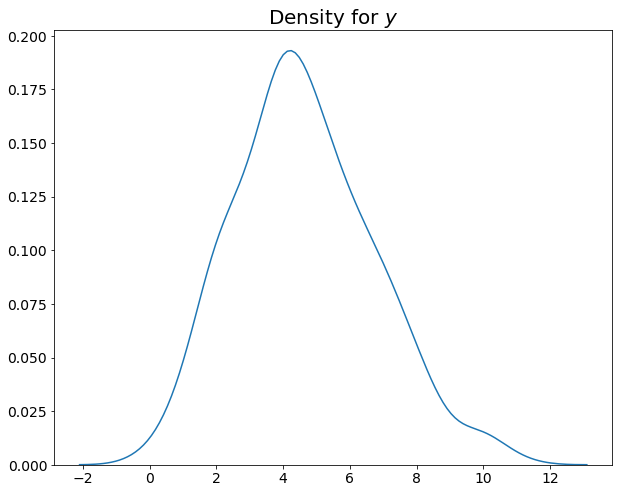
\includegraphics[scale = 0.3]{2a_true_dens.png}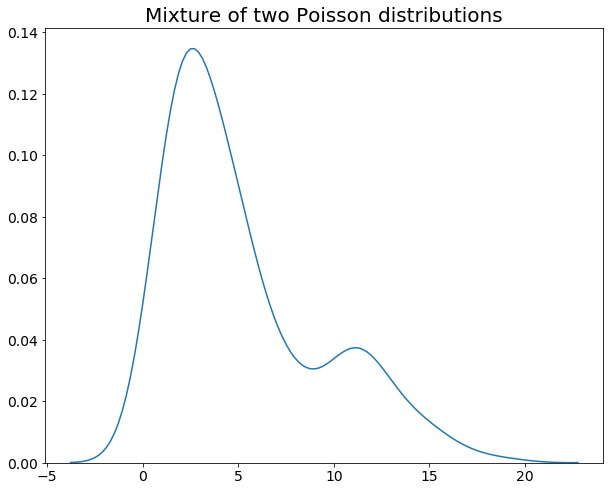
\includegraphics[scale = 0.3]{2b_true_dens.png}
        \caption{Simulated date for a Poisson distribution with mean 5 (left) and simulated data for a mixture of two Poisson distributions with means 3 and 11, and corresponding mixture weights given by 0.7 and 0.3.}
        \label{sim_data_2}
    \end{figure}
    Note, I will use the shape and rate parameterization in the prior Gamma distributions. In other words,
    \begin{align*}
        \alpha &\sim Gamma(1, 0.1)\\
        \lambda &\sim Gamma(5, 1)
    \end{align*}
    The shape 1 and rate 0.1 used in the Gamma prior for $\alpha$, corresponds to a mean of 10 and variance of 200. This allows weight to be given to higher values of $\alpha$ while keeping $\alpha$ low, which is important for the case where the data is not unimodal. Using a unimodal Poisson centering distribution in the DP with low $\alpha$ will allow us to sample more from the empirical distribution of the data and less from the centering distribution. The shape 1.25 and rate 0.25, used in the Gamma prior for $\lambda$, corresponds to a mean of 5 and variance of 5. These are reasonable because the simulated data ranges between 0 and 30.
    
    We can explore the posterior distributions of $F, \alpha$ and $\lambda$ by Gibbs sampling algorithm. At each step, we update $F$ by noting that the DP is a conjugate prior. $F_{new}$ is updated following a $DP(\alpha_{current} + n, \stackrel{\sim}{F_0}(\cdot))$, where 
    \begin{align*}
        \stackrel{\sim}{F_0}(\cdot) &= \frac{\alpha}{\alpha + n} F(\cdot|\lambda) + \frac{1}{\alpha + n} \sum_{i=1}^n \delta_{y_i}(\cdot)
    \end{align*}
    To update the hyper parameters $\alpha$ and $\lambda$, we can use the following to compute the marginal likelihood for DP priors with discrete baseline distributions
    \begin{align*}
        L(\alpha, \lambda; \text{data}) \propto \frac{\alpha^{n^*}}{\alpha^{(n)}} \prod_{j = 1}^{n^*} f_0 (y_j^*|\lambda) \left\{ \alpha f_0(y_j^*|\lambda) + 1 \right\}^{(n_j -1)}
    \end{align*}
    where $f_0(\cdot|\lambda)$ is the p.m.f of $F_0(\cdot|\lambda)$, $n^*$ is the number of distinct values in $(y_1,...,y_n)$, $\{ y_j^*: j = 1,...,n^* \}$ are the distinct values in $(y_1,...,y_n)$, and $n_j = |\{ i: y_i = y_j^*\}|$, for $j=1,...,n$. Using this marginalized likelihood, we can use a Metropolis within Gibbs step to update our parameters in blocks using a multivariate normal proposal distribution. We compute the acceptance ratio based on the ratio of the product of the likelihood and prior evaluated at the proposed candidate and the previous value for the hyper parameters.
    \begin{figure}[h!]
        \centering
        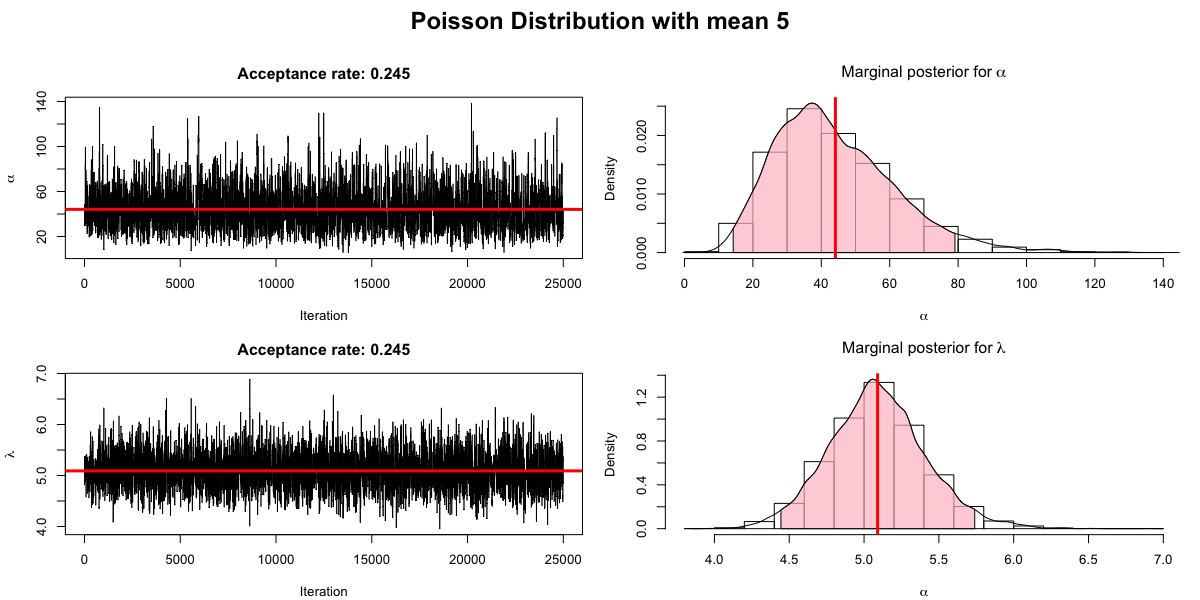
\includegraphics[scale = 0.3]{2a_marginals.png}
        \caption{Left: Convergence trace plots of the marginal posterior distributions for $\alpha$ and $\lambda$ with corresponding acceptance rates. Right: Kernel density estimates for the marginal posteriors, with mean (red line) and 95\% HPD intervals, represented by the pink shaded region.}
        \label{marg_posts_a}
    \end{figure}
    
    \begin{figure}[h!]
        \centering
        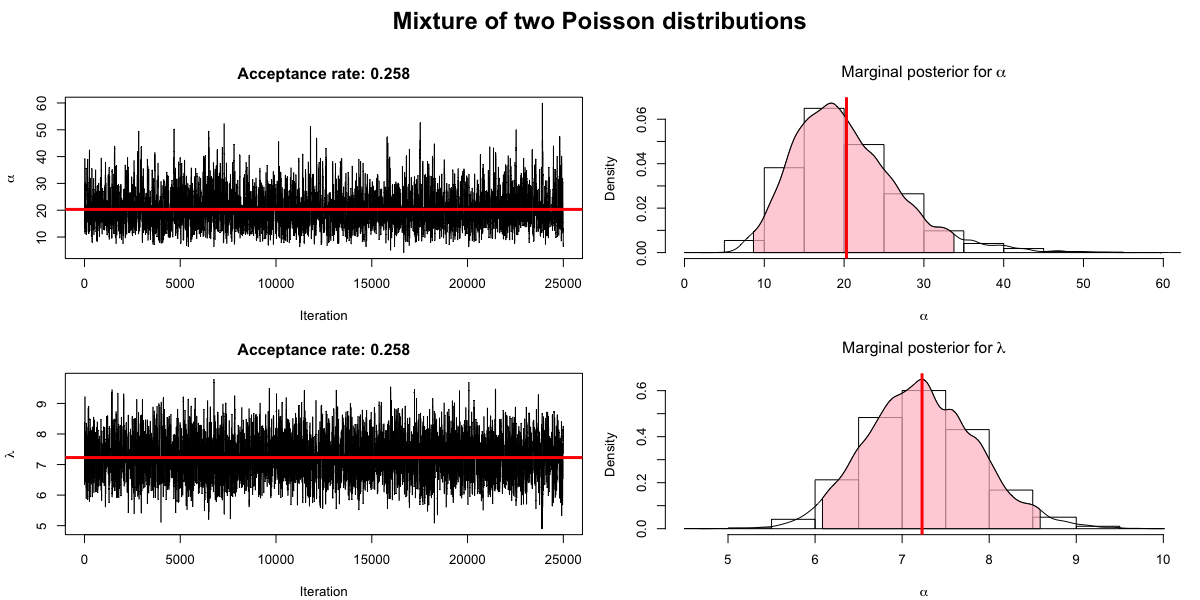
\includegraphics[scale = 0.3]{2b_marginals.png}
        \caption{Left: Convergence trace plots of the marginal posterior distributions for $\alpha$ and $\lambda$ with corresponding acceptance rates. Right: Kernel density estimates for the marginal posteriors, with mean (red line) and 95\% HPD intervals, represented by the pink shaded region.}
        \label{marg_posts_b}
    \end{figure}
    \clearpage
    We obtain point estimates for the two underlying data generating probability mass functions through the posterior predictive distribution. To obtain a posterior distribution $F(y)|\text{data}$, we take our MCMC samples from the joint $p(\alpha, \lambda) \propto \pi(\alpha) \pi(\lambda) L(\alpha, \lambda; \text{data})$   In both cases, the DP recovered the underlying distribution.
    \begin{figure}[h!]
        \centering
        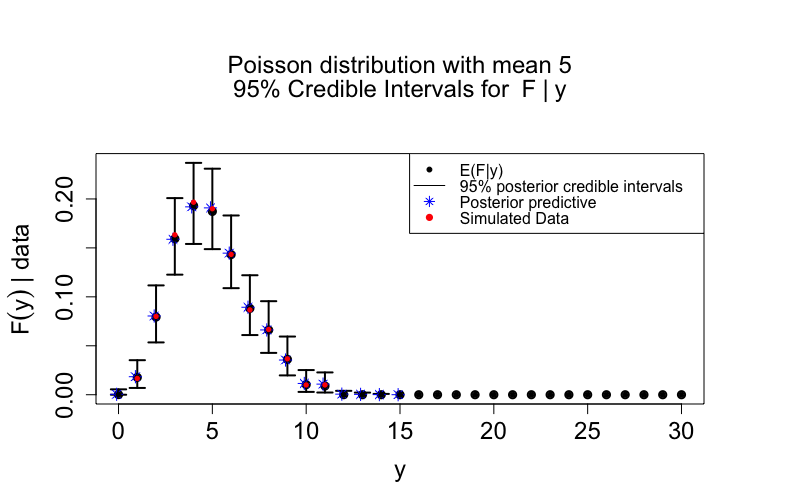
\includegraphics[scale = 0.4]{2a_Posterior.png}
        \caption{The result is that our posterior distribution very closely compares to the data.}
        \label{2a_post}
    \end{figure}
    \begin{figure}[h!]
        \centering
        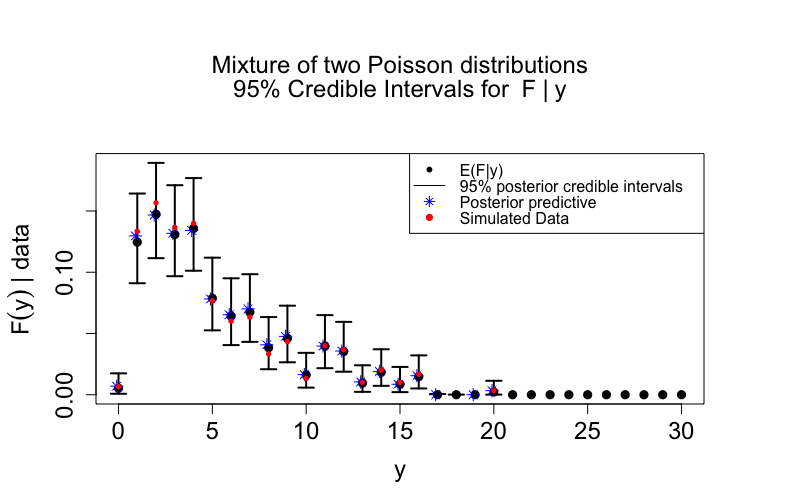
\includegraphics[scale = 0.4]{2b_Posterior.png}
        \caption{Again, the result is that our posterior distribution very closely compares to the data. As with problem 1, the variability can be reduced at each point by increasing $n$.}
        \label{2b_post}
    \end{figure}
    
    

\end{enumerate}
\end{document}